 % !TEX root = ../imprimante3d.tex

\section{Logiciel}

Ce chapitre reprend les grandes lignes des logiciels permettant de convertir un objet 3D en Gcode pour l'imprimante. Nous verrons ensuite plus en détail le logiciel Cura d'Ultimaker. L'objet 3D à imprimer doit être au préalable dans un format standard tel que STL ou OBJ. N'importe quel logiciel de modélisation 3D devrait être capable d'enregistrer ou d'exporter un objet dans l'un de ces deux formats.

\subsection{Concepts}

Voici quelques concepts qu'il faudrait connaitre pour bien paramétrer sont imprimante. Si vous n'utiliser pas les logiciels en mode expert et que vous n'utilisez que les options de base, passez votre chemin.

\subsubsection{Qualité}

La qualité d'une impression dépend surtout de l'imprimante en elle-même. Cependant on peut jouer avec la hauteur des couches pour avoir une meilleure qualité. Pour un brouillon, on peut mettre $2.5mm$, pour une qualité normal, on mettra plutôt $2mm$. Pour une bonne qualité, on utilise $1mm$. On peut aller plus bas encore, mais cela ne change plus grand chose. Il faut savoir que plus les couches sont fines, plus il faudra en faire et donc plus l'impression sera longue.

\paragraph{} Si l'objet ne parait pas assez remplis sur les couches inférieures ou supérieur, le flux est peut-être mal régler. On peut changer le flux directement pendant une impression avec le contrôleur (pour l'Ultimaker du moins). Sinon on peut jouer avec les paramètres de diamètre et densité du filament pour avoir plus ou moins de matières déposées à chaque passage.

\subsubsection{Vitesse}

Une vitesse standard pour une impression est autour de $50mm/s$. La encore une fois tout dépend de l'imprimante. L'Ultimaker peut aller facilement jusqu'à $150mm/s$ du fait se sont faible poids de sa tête (dû à l'extrudeur placé en dehors). Une grande vitesse pourra avoir une influence négative sur la qualité de l'objet. Pour l'ultimaker une vitesse de $80mm/s$ est une bonne valeur.

\paragraph{} Dans les paramètres avancés, on peut également régler la vitesse de la première couche. Cette couche est très importante vue qu'elle sera responsable de l'adhésion de la pièce. Une vitesse inférieure à la vitesse normale d'impression est donc appliquée. Une vitesse de $20mm/s$ est une valeur standard pour la première couche.

\subsubsection{Adhésion}

Dans certains logiciels comme curra, il est possible d'utiliser une technique d'adhésion particulière. Ces techniques servent à ce que la pièce tienne bien en place sur le plateau. Il est très important d'en ajouter une quand la pièce est grande, mais que la surface d'adhésion est petite.

\begin{description}
\item [Brim] ajoute plusieurs lignes tout autour de la pièce. On peut facilement enlever cette couche supplémentaire sans pour autant détériorer la pièce. 
\item[Raft] ajoute un \emph{radeau} sous la pièce. Fonctionne bien, mais il faudra raboter le fond de la pièce après l'impression. L'état de surface ne sera pas forcément très lisse.
\end{description}

Dans la plupart des cas, on utilise \emph{brim}.

\begin{figure}[H]
	\centering
	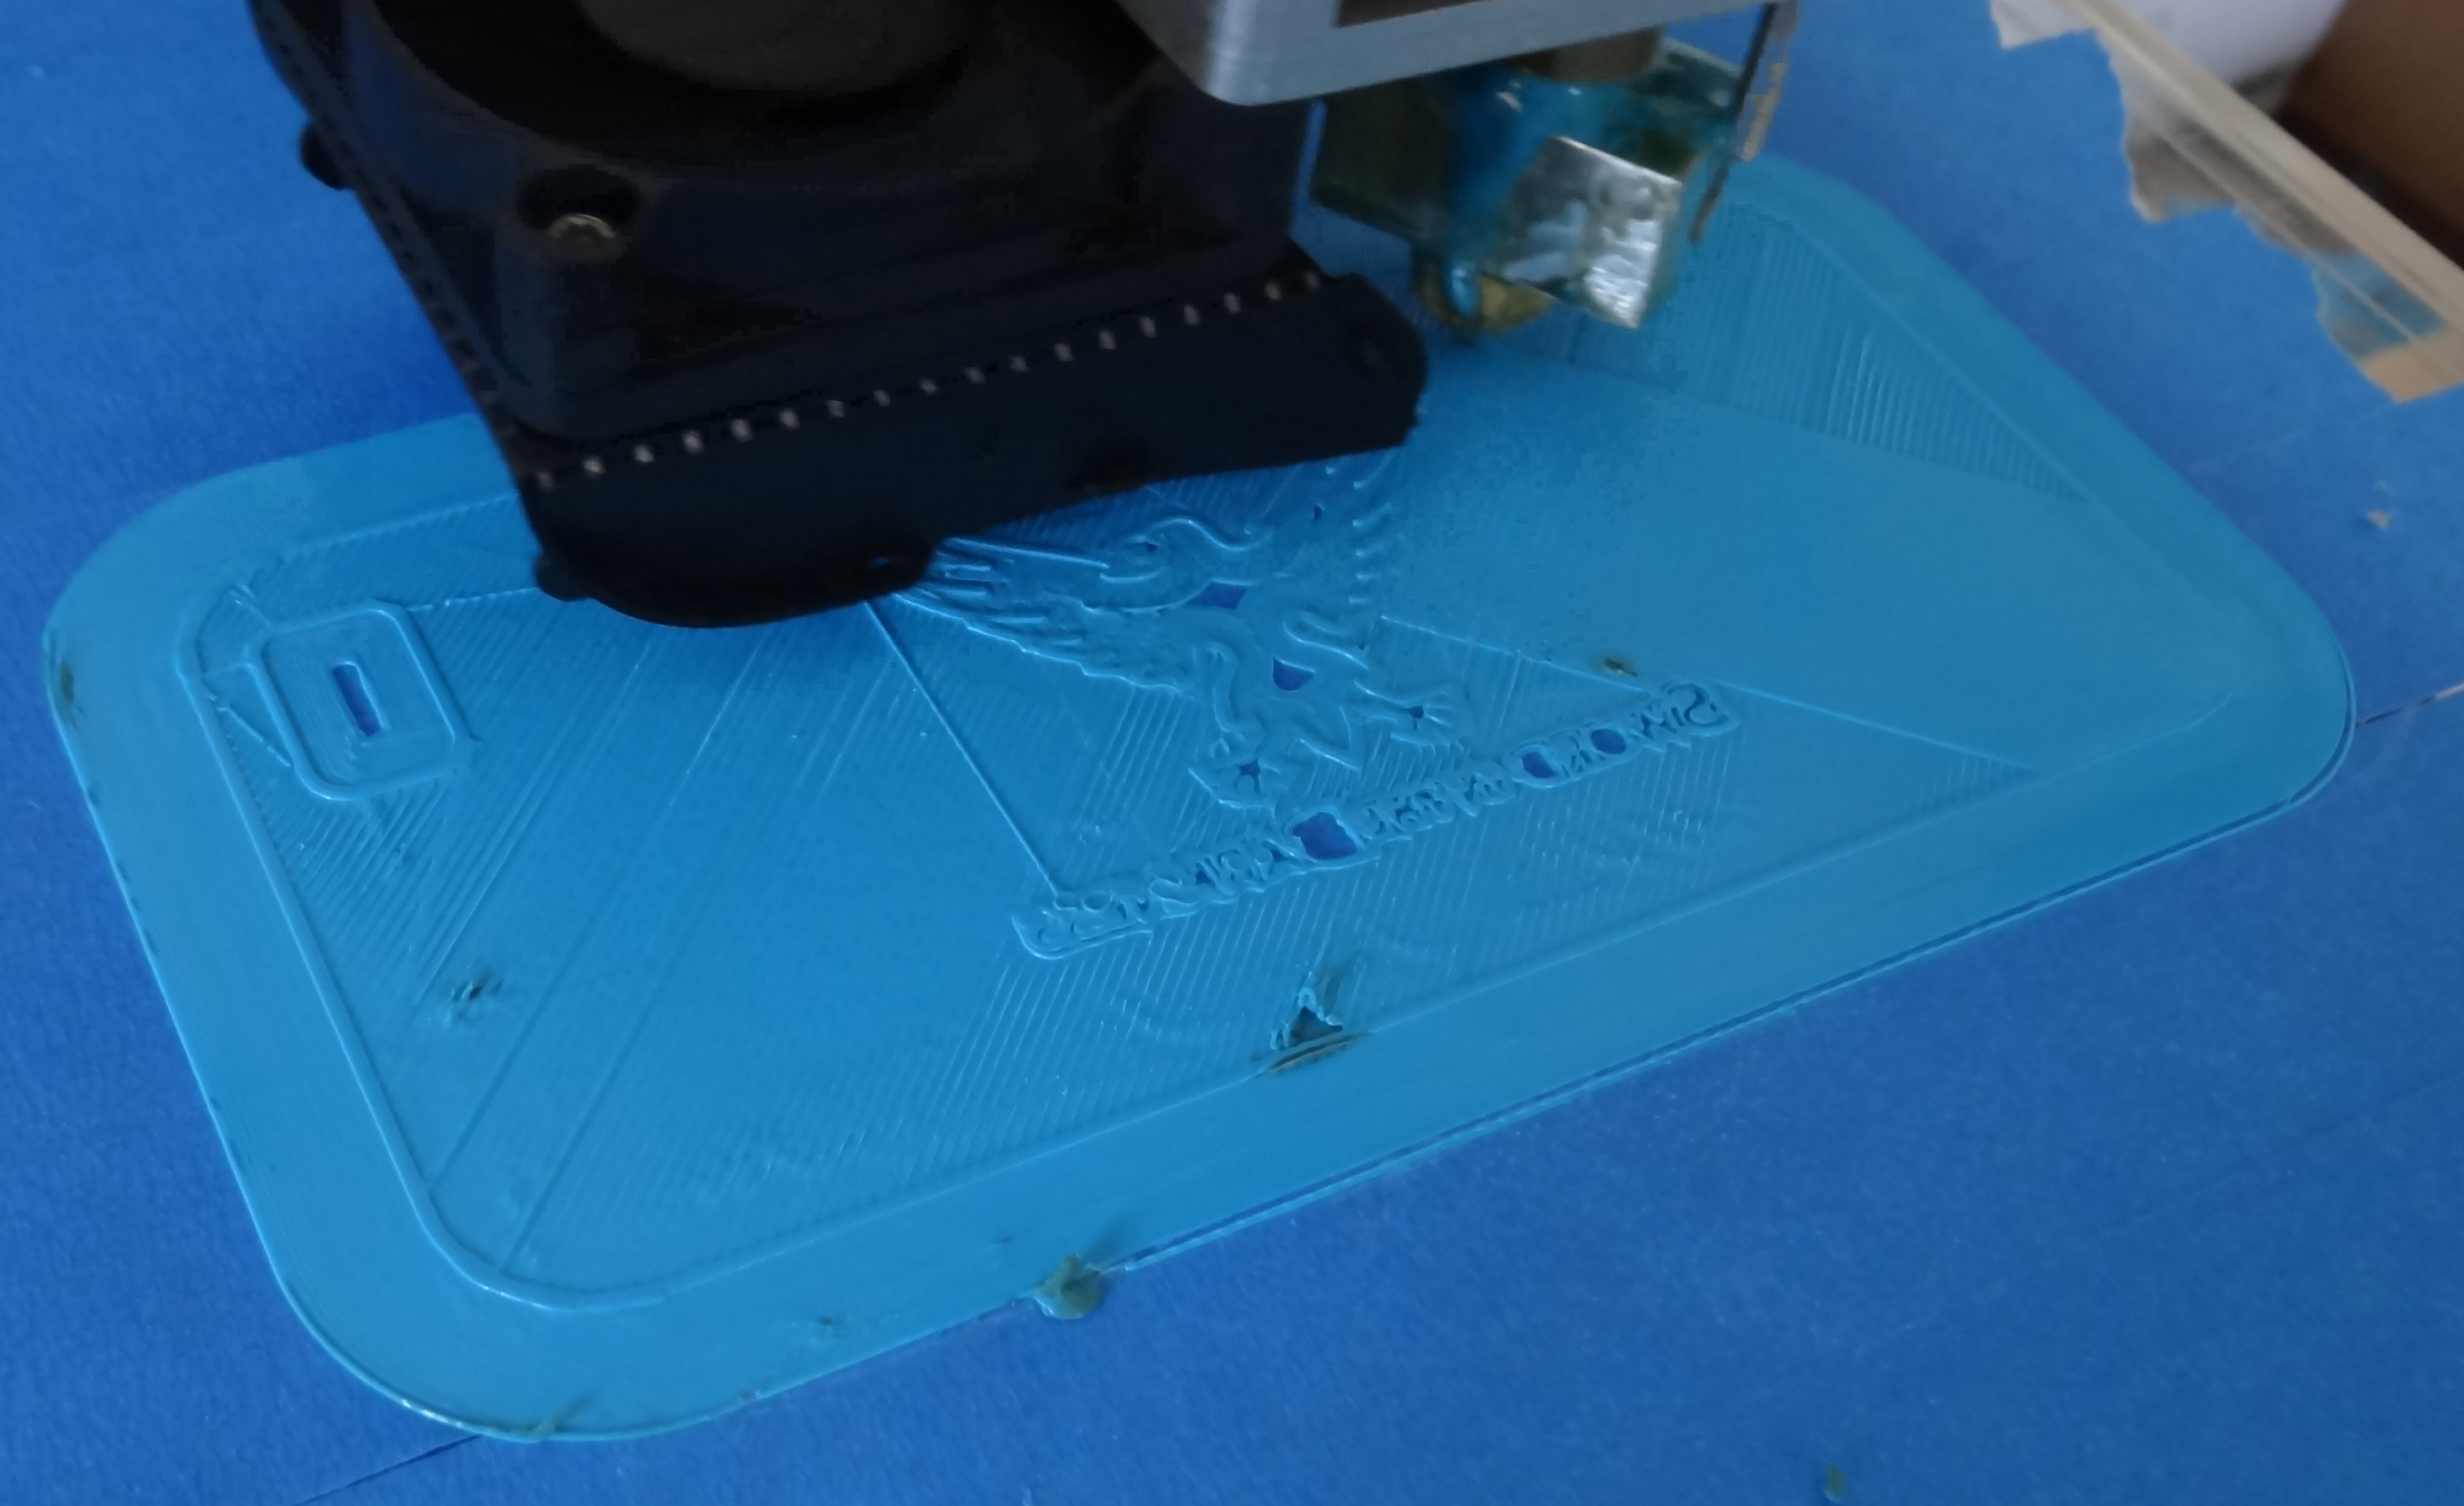
\includegraphics[width=50ex]{03_logiciel/brim.jpg}  
	\caption{Adhésion : brim}
	\label{fig:brim}
\end{figure}

Sur la figure \ref{fig:brim} on peut clairement voir qu'une couche à été rajouter tout autour de l'objet (ici, une coque d'Iphone).

\subsubsection{Support}

Une imprimante 3D imprime de bas en haut. S'il arrive que pour un objet on doive démarré l'impression d'une de ses parties dans le vide, il faut ajouter un support. Ce support pourra être facilement enlevé après l'impression. Il y a plusieurs types de support :

\begin{description}
\item [Touching buildplate] Ajoute un support uniquement entre le plateau et la pièce (si besoin)
\item[Everywhere] Ajoute en plus un support à l'intérieur de la pièce (si cela est nécessaire)
\end{description}

Il n'y a pas de valeur par défaut ici, il faut voir au cas par cas. Mais pour le $90\%$ des pièces, aucun support n'est requis.

\subsection{Cura}

\subsubsection{Mode}

\begin{description}
\item [Quickprint] (Impression rapide) Ce mode ne permet que de choisir entre bonne, normale et basse qualité. Cura adaptera tous les paramètres pour vous. On peut voir ça comme un mode automatique
\item[Full settings] (Toutes les options) Ce mode donnes accès à tous les paramètres avancés de l'application.
\end{description}

\subsubsection{Paramètres}
Sur la gauche de Cura se trouvent les paramètres d'impression. Ils ne seront pas tous détaillés ici. On retrouve notamment les paramètres des concepts expliqués précédemment.

\subsubsection{Différentes vues 3D}
La vue 3D nous donne une vue de l'imprimante et de la pièce que l'on va imprimer. La couleur n'a bien entendu rien à voir, elle dépend uniquement du filament installé.

\paragraph{} En haut à droite, on a un bouton pour choisir le type de vue que l'on veut. Une vue qui peut s'avérer utile est la vue \emph{Layers} (couches). Elle montre couche par couche la trajectoire que Cura a calculée.


\subsubsection{Éditer la pièce}

Nous pouvons éditer basiquement la pièce directement depuis Cura. C'est-à-dire que nous pouvons l'agrandir ou rétrécir (\emph{Scale}), nous pouvons la retourner (\emph{Rotation}) et nous pouvons lui appliquer des effets de miroir (\emph{Mirror}). Toutes ces actions peuvent être effectuées à l'aide des boutons en bas à gauche de la Vue 3D.

\subsubsection{Exporter pour imprimer}

A l'aide des boutons en haut à gauche, nous pouvons enregistrer le GCode (le code machine). Le Gcode peut-être placé sur une carte SD pour ensuite être introduite dans le contrôleur. Si l'imprimante est directement connectée, on peut également lancer l'impression directement depuis Cura.

\subsubsection{Estimations}

Cura estime le temps d'impression, le poids de la pièce et les mètres de filament requis. Ces valeurs sont à prendre avec des pincettes. Elles sont très souvent inférieures à la réalité. Pour le temps, on peut parfois compter jusqu'au double pour les très petites pièces. Pour une pièce de taille moyenne, le temps d'impression peut faire jusqu'à $50\%$ plus longtemps. Néanmoins, cela nous donne un ordre de grandeur, et surtout, cela nous permet de comparer les changements en fonction des parères que nous voulons. 

























